\part{ECL Programming}

\chapter{Introduction}

ECL is a declarative language that can be used to work with huge data projects, in the HPCC platform. Its most powerful feature is that you can re-use each query for every subsequent queries. Here's a sample program (It is part of the ECL Playground sample code).

So, breaking it down, there are two types of ECL Code: Definitions, which define what is to be done (eg. loading up a dataset, sorting through a part of a file, and so on) and actions, which are, well, actions; they define what are the actions that are required. Here's a sample program that is from the ECL Playground (most likely the first thing you will see when you load up the playground):

\lstinputlisting[caption={(P0) Comments, Definitions, and Actions},firstline=5]{../source/00-eclStarter.ecl}

The first thing to keep in mind, is that ECL, is \textbf{case-insensitive}. Comments are done in a C/C++ fashion of \lstinline!//! as line-comments and \lstinline!/* */! as block comments. It uses the standard \lstinline!object.property! structure and can be use to nest definitions neatly (Note that it is not an object oriented language).

Execution in ECL, is done by following the trail given by the actions. The execution of an action, requires definitions, which are compiled and executed accordingly. Note that this implies that there \textbf{may not be} an explicit execution order; execution is reordered in a way that helps speed up execution.

Consider the example above, it consists of three definitions, one record, one dataset, and one last definition which is a filter of the previous dataset.
The final line is an action which creates the execution graph. (This is a great segway into the next section.)
\pagebreak
\section{Graph Solver}


% \begin{wrapfigure}{r}{3.5cm}
    %     \begin{center}
        %         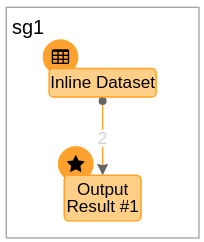
\includegraphics[width=3.4cm]{../media/simplegraph.png}
        %     \end{center}
        %     \caption{\tiny{Graph for (P0)}}
        % \end{wrapfigure}
        
ECL can actually be considered an optimized graph solver. Digging into ECL Watch, we can obtain this pretty (simple) graph for that previous code sample:
\begin{figure}[h]
    \centering
    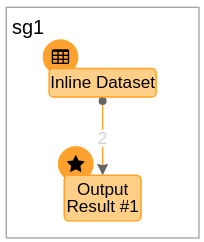
\includegraphics[height=3.5cm]{../media/simplegraph}
    \caption{Graph for (P0)}
\end{figure}

Each node is some activity, and the (computation) graph is solved in the best possibly way in ECL. The fact that the computation can be very well optimized by mentioning "what" to do, rather than "how" to do, presents a lot of speedups and the ability to parallelize the program as much as possible.

Look at this other example, for which the source code is given:

\lstinputlisting[caption={Source code for the graph below (Don't worry about what's in the code)},firstline=2]{../source/01-graph2.ecl}

\begin{figure}[h]
    \centering
    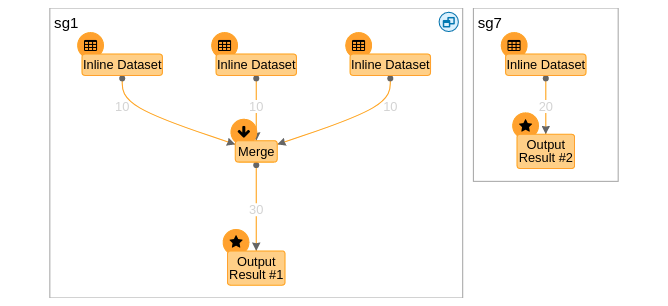
\includegraphics[width=.6\linewidth]{../media/bitlesssimplegraph.png}
    \caption{Bit less simple graph}
\end{figure}

The program above, has two outputs (actions). In this case, two graphs are generated and can be executed accordingly, independently from each other as required. Using this idea, the ECL compiler will compile this ECL code into C++ code that can then be executed on a cluster. This mindset of "graphs" is rather important to the understanding of ECL, as this will help differentiate it from the traditional imperative style of programming.

% \pagebreak
\section[Chapter information and Datasets]{A rundown of the chapters and datasets used}

The other chapters give examples in ECL, their outputs, and (hopefully) a good understanding of how they work. The last chapter, gives some key methodologies in ECL that is necessary/useful for Machine Learning.

Datasets used have been provided, and can be referred to from the provided repository \url{https://github.com/chrisvrose/bda6-ecl-basics}. Record structures will be given as per the examples, but some corresponding records are also provided for reference.

There are 4 datasets of importance to note:
\begin{enumerate}
    \item heart\_failure.csv - A dataset having 13 attributes of a patient, and whether they have heart disease or not. Refer to the \href{https://www.kaggle.com/ronitf/heart-disease-uci}{kaggle page} for more data. 
    \item house\_prices\_data.csv - A dataset that shows the price of a house, given key attributes about it. Refer to the \href{https://www.kaggle.com/shivachandel/kc-house-data}{user's submission on kaggle} for more data.
    \item Salary\_Data.csv - Years of Experience vs Salary. Its the smallest dataset, and undoubtedly the simplest.
    \item Social\_Network\_Ads.csv - Similar to the earlier dataset, but includes some additional attributes.
    \item vocab.enron.txt - This is a set of words that is used often in machine learning, from the \href{https://archive.ics.uci.edu/ml/datasets/Bag+of+Words}{UCI Machine Learning Repository}
\end{enumerate}

The scope expected in the programs given below is `\~{}eclbasics', but the reader is free to configure them accordingly.


\subsection{Running ECL programs}

The best way to run these, is to first upload and spray the data accordingly, and submit the script using your ECL Client Tools. If using VSCode, an extension is available which uses the Client Tools (On Windows, don't forget to add \lstinline{ecl} to the PATH variable. The target, is left to the reader to pick accordingly (although these have been tested on \lstinline{thor} and \lstinline{hthor}).

\chapter{Basics}

\section{Data Types}

ECL has a list of basic data types, but more may be derived by the developer.
Some common datatypes are enumerated below. (Use this for quick reference)
\begin{table}[h]
\centering
\begin{tabular}{|c|c|}\hline
Data Type & Description \\\hline\hline
STRING[n] & Packed (or null-terminated) string \\
UTF8 & Unicode character string \\
UNICODE[\_locale][n] &  UTF-16 encoded unicode character string \\
INTEGER[n] & n-byte integer value n can be: 1 - 8 \\
UNSIGNED[n] & n-byte unsigned integer value \\
REAL[n] & n-byte IEEE floating point value \\
DECIMAL\textlangle{}n\textrangle{}[\_y] & Packed decimal value of n total digits \\
BOOLEAN & Boolean value \\
SET OF \textlangle{}type\textrangle{} & A set of values\\
RECORD & Ordered collection of data (Like a tuple)\\
DATASET & Collection of records \\\hline
\end{tabular}
\caption{Common Data Types}
\end{table}

These data types are used very frequently, and more documentation can be found in the \href{https://hpccsystems.com/training/documentation/learning-ecl}{HPCC Systems Learning ECL} page. Following subsections will start with some programs and how they work.

Additionally, in ECL, data types are \textit{inferred} from the assignment if possible. This means that writing

\lstinline{STRING a:= 'Hello';} and 

\lstinline{a:= 'Hello';}

\noindent{}are both giving `a' a type \lstinline{STRING}. 

Other than these basic data types, definitions may also be \lstinline{MODULE}s and \lstinline{FUNCTION}s. These are explored in later sections.

\section{Working with ECL}

\subsection[Simple Statistics on Datasets]{(P1) Reading up a dataset and finding some very simple statistics on it}

Scenario: We have a dataset `Salary\_Data.csv', and we want some basic stats on it as sanity checks, before we do some actual work on it. Let's get four things about it:

\begin{enumerate}
    \item Count of rows
    \item Avg years of experience in the dataset
    \item The maximum and the minimum salary that was obtained
    \item The first entry of the dataset.
\end{enumerate}

\lstinputlisting[caption={Program 1 - Sanity checks}]{../source/12-meagre-stats.ecl}

\pagebreak
The output is shown here in XML, but later examples may be shown as table pictures based on the amount of outputs from the program.
This XML output gives a nice description and structure to the output. The result is shown as a set of datasets, which have rows, where values are shown as labelled items.

Some important things to note here, is that ECL arrays, are one-indexed and not zero indexed, like most popular languages. 
Additionally, the `+' operator can perform set operations as well, which we can talk about more later on.
\lstinputlisting[caption={Output 1 - Sanity checks},language=xml]{../output/12/output.xml}



\subsection{Datasets and Records}

\subsubsection[Common data operations]{(P2)Loading up a dataset and working with it}

Being able to filter and process data is rather important. This program should illustrate the common operations that can be done in ECL. This, includes horizontal slicing (filtering), vertical slicing (column-based filters).


\lstinputlisting[caption={(P2)Dataset operations}]{../source/26-common.ecl}


Result 2 and 'projections' will look similar, and that countofYoung is zero. Its an interesting thought, as both can be used for our goal here, but the latter method using projections allow us to refer it later by assigning it to a definition (You can assign an action to a definition, but that is not the same as this). It should also be noted that the \lstinline{TABLE} function can provide a functionality similar to this too, and its functionality is shown later.

Here's the rest of the outputs:

\begin{figure}[h]
    \centering
    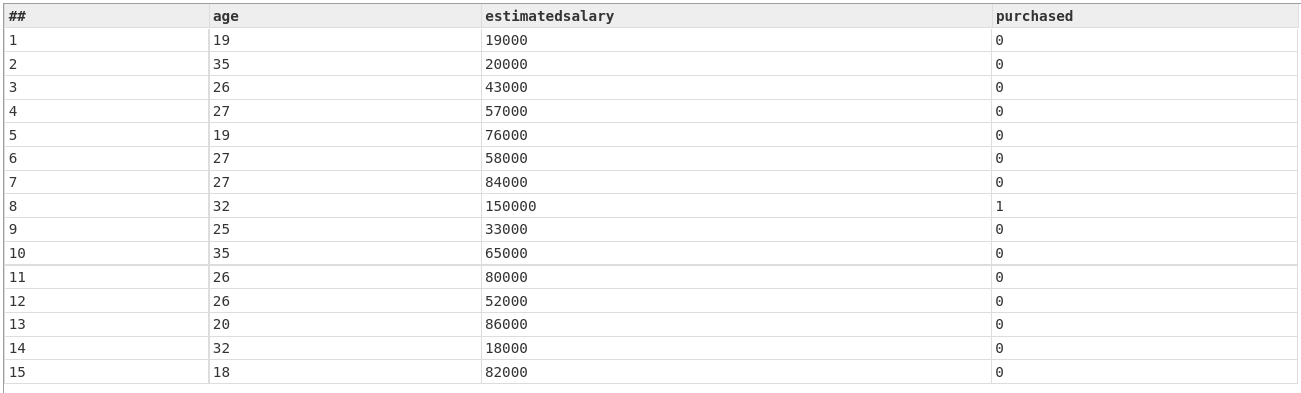
\includegraphics[width=\linewidth]{../output/26/1.png}
    \caption{Result 1 - Output of a segment}
\end{figure}


\begin{figure}[h]
    \centering
    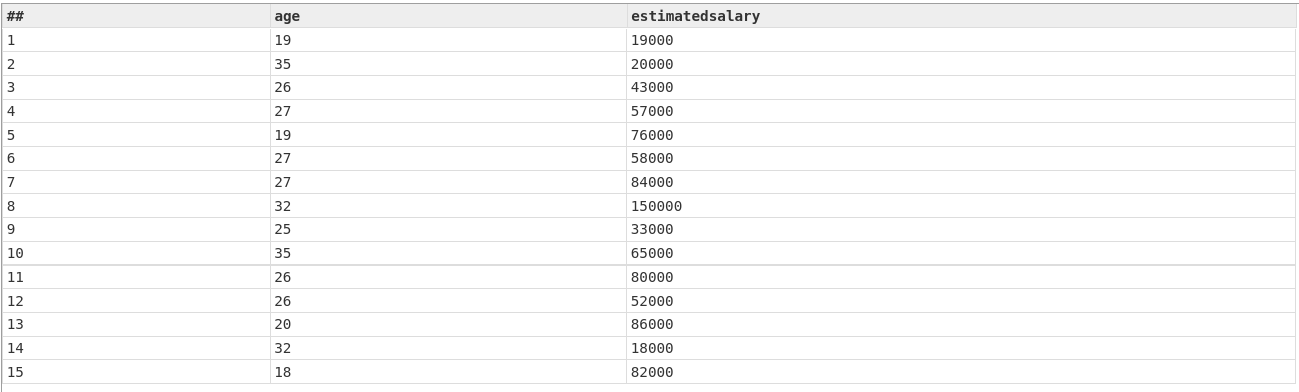
\includegraphics[width=\linewidth]{../output/26/2.png}
    \caption{Result 2 - Output, filtering columns (Only age and salary here)}
\end{figure}

\begin{figure}[h]
    \centering
    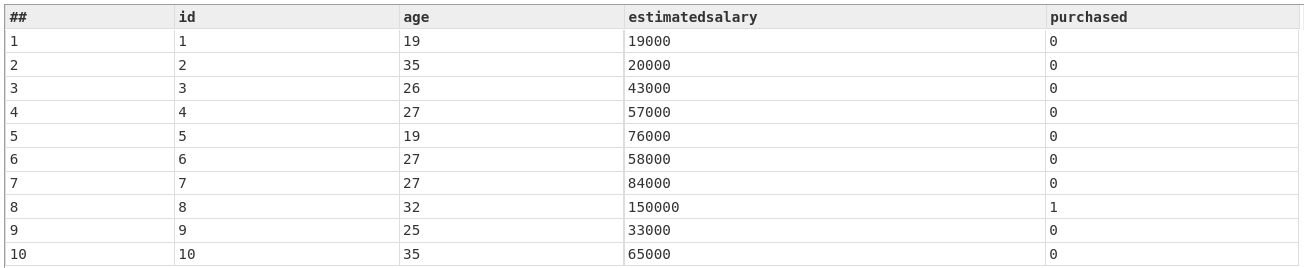
\includegraphics[width=\linewidth]{../output/26/6withid.png}
    \caption{Result 6 - Adding ids with transforms}
\end{figure}


\subsubsection[Filtering \textit{n}\textsuperscript{th} record]{(P3)Filtering by nth record}

Filtering by the nth record is not as unusual as it might look. In ECL, datasets, statements may not may not be order-sensitive, and can be configured as such. This means that the order of the dataset, cannot be ignored, and can be used (Unlike 1NF normalized databases where record positions should never matter).
For a case of \lstinline!n=2!, this problem devolves into picking out every 2nd number, ie. even numbered item.

Let's try the same on \lstinline!Social_Network_Data.csv!, with $n=3$.


\lstinputlisting[caption={(P3) Filtering to n-th record}]{../source/27-nth.ecl}

The output looks rather standard, and there are 134 records output (That's output 2, which is not shown here).

\begin{figure}[h]
    \centering
    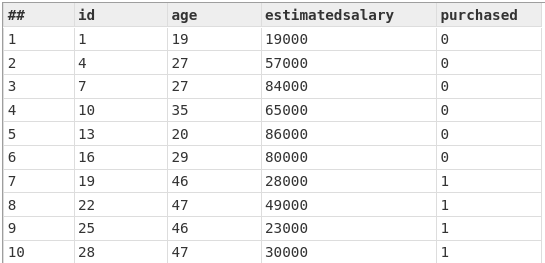
\includegraphics[width=.75\linewidth]{../output/27/1filt_op}
    \caption{Result 1 - Notice that the ids print only the 3rd record}
\end{figure}
\pagebreak
\subsection{Deduplication \& Normalization}

\subsubsection{Deduplication}

For data manipulation, data normalization and dedup play a very large role too. \lstinline{DEDUP} in ECL is a bit special in that you can specify the kind of deduplication wanted. As record order can be made significant; DEDUP can perform dedups locally or over the whole dataset.
The best way to work with \lstinline{DEDUP} is to first sort your data before feeding it to DEDUP. Options for KEEP and BEST can be used for more fine-grained control over how the output dataset will be made.

\lstinputlisting[caption={(P4) Dedup}]{../source/29-dedup.ecl}

The output, is shown here in csv, and looks like:

\lstinputlisting[caption={(P4) Deduplication - Output 1}]{../output/29/WUResult.csv}
\lstinputlisting[caption={(P4) Deduplication - Output 2}]{../output/29/WUResult (1).csv}
\lstinputlisting[caption={(P4) Deduplication - Output 3}]{../output/29/WUResult (2).csv}
\lstinputlisting[caption={(P4) Deduplication - Output 4}]{../output/29/WUResult (3).csv}



\subsubsection{Normalization}

The \lstinline{NORMALIZE} function `normalizes' child records out of a recordset where the child records are appended to the end of the parent's data records. The purpose is to take a variable-length flat-file recordset, and split out the child information. For those coming from a Spark or JS background, it can be thought of as the \lstinline{.flatMap()} operation. 

Below is one of the two forms of \lstinline{NORMALIZE}.

\lstinputlisting[caption={(P5) Normalize}]{../source/28-normalize.ecl}

The output record, looks like:

\begin{figure}[h]
    \centering
    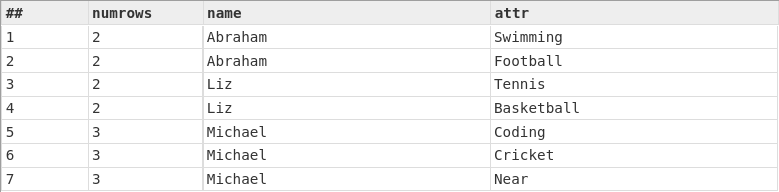
\includegraphics[width=.8\linewidth]{../output/28/1}
    \caption{Result 1 - NORMALIZING}
\end{figure}

\subsection{Iteration \& Recursion}

Functions, unfortunately, may not be called from itself in ECL. This removes the idea of recursion, in ECL.
Instead, we can attempt to use \lstinline{LOOP} to apply tranformations to a dataset.


\subsubsection{(P6) Fibonacci numbers}

\noindent{}Fibonacci sequence generation is a classic iteration/recursion program.
\lstinputlisting[caption={(P6) Fibonacci}]{../source/43-fibonacci.ecl}

The \lstinline!LOOP! function be used to perform an operator multiple times. Note that in this body, the COUNTER keyword is implicitly available for use.

For each successive iteration of \lstinline{LOOP}, the input dataset is the result set of the previous iteration. Let's take a look at the output of the program below.

\begin{figure}[h]
    \centering
    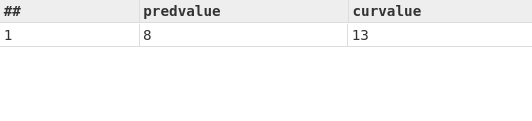
\includegraphics[width=.6\linewidth]{../output/43/op.png}
    \caption{(P6) Output}
\end{figure}

In fact, we can get the final value out of the set by catching the curvalue of the first element of the dataset.

\subsubsection{(P7) Factorial}

A simpler example for how loop works, is the factorial. \lstinline!LOOP! can be used to get the $n!$.
Here's a program and a sample output:

\lstinputlisting[caption={(P7) $10!$}]{../source/44-factorial.ecl}

\begin{figure}[h]
    \centering
    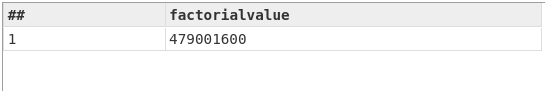
\includegraphics[width=.6\linewidth]{../output/44/1.png}
    \caption{(P7) Output 1}
\end{figure}


\subsection{Denormalization}

Denormalization is the reverse of normalization (thankfully the name suggests that too). Here, a combined record is made out of a \textit{parent} and any number of \textit{children}. Its somewhat like a \lstinline{JOIN}, which will be seen later, but whereas the latter produces n outputs given 1 parent and n children, DENOMRALIZE runs the transformation fucntion and produces only one output. As DENORMALIZE is essentially a specialized form of JOIN, the various join types (LEFT OUTER, RIGHT OUTER, FULL OUTER, LEFT ONLY, RIGHT ONLY, FULL ONLY) are also available for use on DENORMALIZE and act just as they do with JOIN. However, we can work without these specificities for the sake of understanding. Note that such a program also requires a transformation function, like all the various operations that we have seen so far.

\section{ECL and SQL}

Data Analysts may find their needs well expressed in ECL as well. ECL can perform powerful aggregations, filtering, sorting, deduplication and expressive visualizations.

% 3 programs
\subsubsection{Basic SQL comparisons}

ALthough SQL is used mostly in databases, it is a popular choice for data querying and analysis. 
Some comparisons are given below to guide those who have prior knowledge of SQL and also to help show the differences in how SQL and ECL can be used given similar objectives.


\lstinputlisting[caption={(P8) SQL and ECL - Basic querying and aggregtions}]{../source/62-sql1.ecl}

Here's how the output looks like:

\begin{figure}[h]
    \centering
    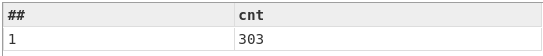
\includegraphics[width=.55\linewidth]{../output/62/1.png}
    \caption{(P8) Output 1 - Number of rows in this dataset}
\end{figure}

\begin{figure}[h]
    \centering
    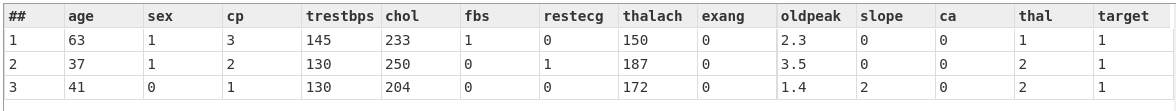
\includegraphics[width=\linewidth]{../output/62/2}
    \caption{(P8) Output 2 - 3 enties of people who have heart disease}
\end{figure}
\begin{figure}[h]
    \centering
    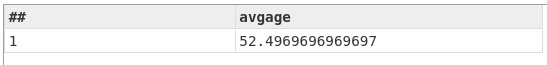
\includegraphics[width=.55\linewidth]{../output/62/3}
    \caption{(P8) Output 3 - The average age of a person who had heart disease}
\end{figure}

\subsection{SQL Queries involving grouping and ordering}

In HPCC Systems, the \lstinline{TABLE} query can also be used to help perform more expressive queries. Grouping and column filtering is possible in one statement here.

\lstinputlisting[caption={(P9) SQL and ECL - Grouping and sorting}]{../source/62-sql1.ecl}

The outputs are as shown:

\begin{figure}[h]
    \centering
    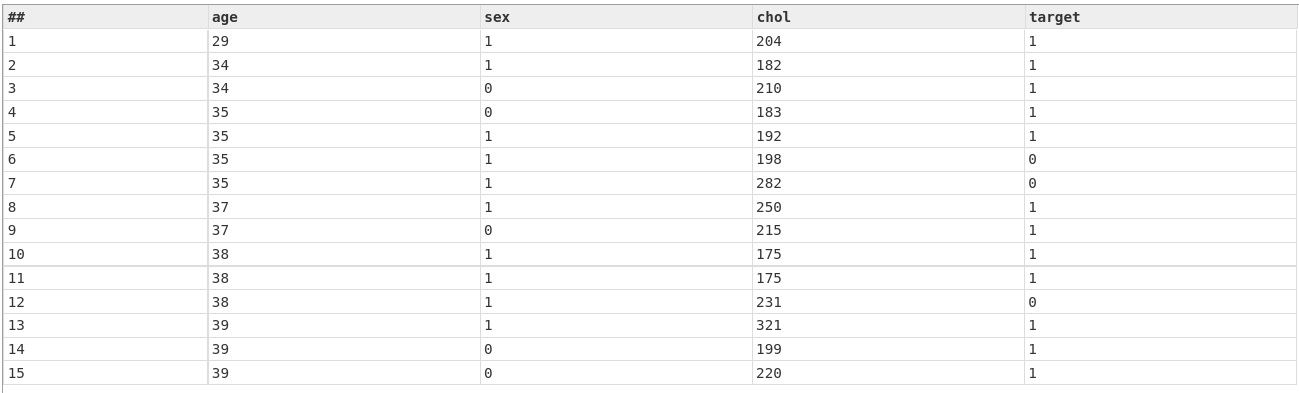
\includegraphics[width=.75\linewidth]{../output/63/1.png}
    \caption{(P9) Output 1 - Information about the youngest few people in this dataset}
\end{figure}

\begin{figure}[h]
    \centering
    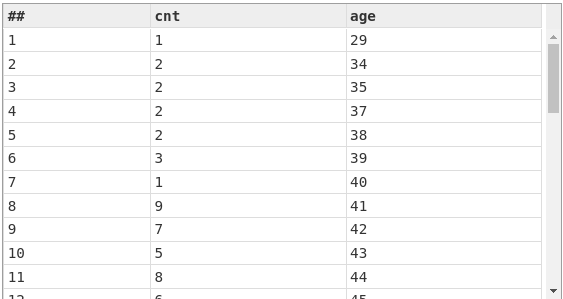
\includegraphics[width=.5\linewidth]{../output/63/2}
    \caption{(P9) Output 2 - A grouped report of age-wise counts of heart disease}
\end{figure}
\begin{figure}[h]
    \centering
    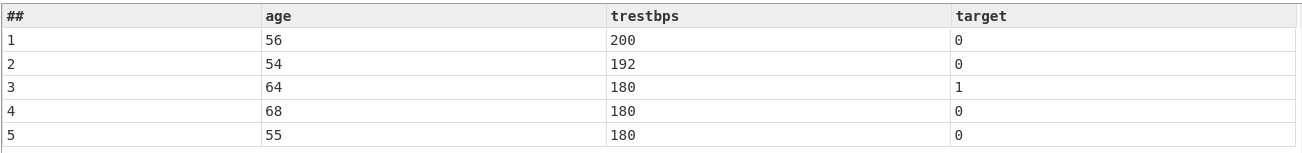
\includegraphics[width=.75\linewidth]{../output/63/3}
    \caption{(P9) Output 3 - The age and the resting heart rate, and whether they had a heart disease, ranked by heart rate}
\end{figure}

\subsubsection{Working with multiple data sources}

SQL queries often support joins to combine data. ECL has the MERGE, and JOIN operators to help with this. Reconsider one of the earlier examples.

MERGE can be used to combine datasets in an efficient manner, although this requires the dataset to be be sorted prior to usage. 
\lstinputlisting[caption={(P10) Merging sorted data},firstline=2]{../source/01-graph2.ecl}

If record order is not constrained, the \lstinline{+} operator may be used. 
However, for constrained based joining of data, JOIN is often used. There are various types of joins, although here only \lstinline{INNER} has been depicted as it is most used. Consider the following example for simple joining.

\lstinputlisting[caption={(P11) Joins}]{../source/64-sql3.ecl}

\begin{figure}[h]
    \centering
    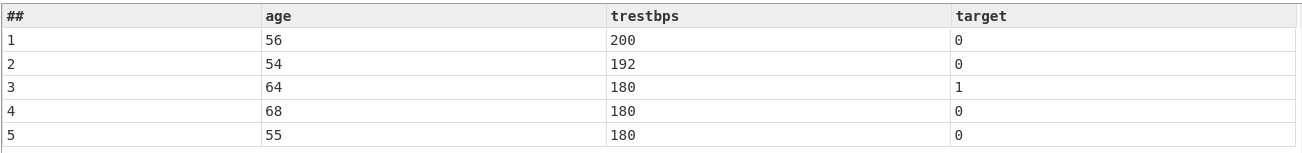
\includegraphics[width=.92\linewidth]{../output/63/3}
    \caption{(P11) Output 1 - Details to bill a person with}
\end{figure}


\chapter{Using Modules}
\section{General module usage}
Modules are a great way to segment your code and split it into separate sections.
Although the \lstinline!.! operator really is reminiscent of OOPs like programming, it is good to remember that ECL does \textit{follow} OOPs.

Consider the following as an example to help explain the various scopes available within a module.
\lstinputlisting[caption={(P12) ./datsrc/modeg.ecl}]{../source/datasrc/modeg.ecl}

\lstinputlisting[caption={(P12) - Using the module}]{../source/75-modules.ecl}

The output, especially showcases the behaviour of default-scoped variables.
\begin{figure}[h]
    \centering
    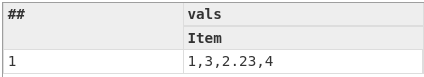
\includegraphics[width=.6\linewidth]{../output/75/1}
    \caption{(P12) Output 1}
\end{figure}

An important point to note is that an ECL program with an export, should not contain actions. This can be understood in the way that export itself is the "output" of the program, ie. the intention of the program is to export these values. This also means that although such programs can be syntax checked, modules cannot be directly executed. However, actions may be tied to definitions and be used in a calling program.


\subsection{Standard library}

The Standard library comes with a lot of very useful functionality for data processing.

\subsubsection[String Handling]{String Handling}

A lot of string handling functions are present as part of the Standard library, and may be used. Note that the \lstinline{TRIM} does not require to be imported from the standard library, even though its primary purpose is string processing.
As a precursor to some other uses, let's consider a case of palindromes, a program that prints out palindromes from a set of words.


\lstinputlisting[caption={(P12) - String handling}]{../source/76-std-stringsimple.ecl}

There are 119 palindromes that come out of our set, and here are a few of them:

\begin{figure}[h]
    \centering
    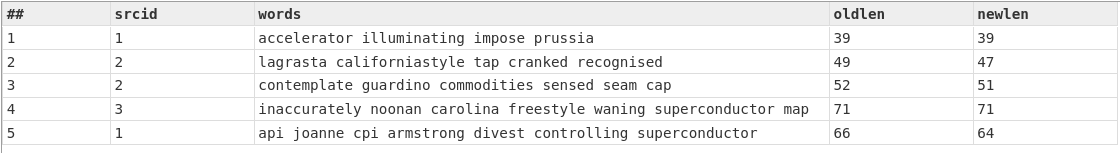
\includegraphics[width=.5\linewidth]{../output/76/1}
    \caption{(P12) Output 1 - Sample of palindromes found}
\end{figure}


The below program recaps some of the earlier concepts on normalize and shows a sample set of data of words, with the objective being to find a set of words which can have some minimal edits to result in the given word.

Right now, the definition \lstinline{word} is hardcoded, but this can be a parameter to a query and this program would extend into a query that would find the minimum edit distance between the words in the dataset.
The final output for 'ap' looks like:

\begin{figure}[h]
    \centering
    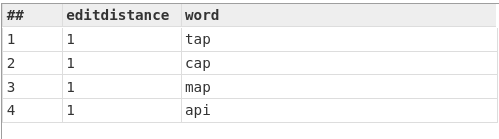
\includegraphics[width=.6\linewidth]{../output/77/5}
    \caption{(P13) Output 5}
\end{figure}

\subsubsection{Date/Time support}

Date Time support is extremely important for any language. The standard library provides a multitude of functions to parse, represent and use date and time values.
Below is a simple example that shows which day of the week today is and what tomorrow is.


\lstinputlisting[caption={(P14) - Date handling}]{../source/78-std-date.ecl}

The output of this program is short, and shows the current date (note that it is pulled in as UTC).

\begin{figure}[h]
    \centering
    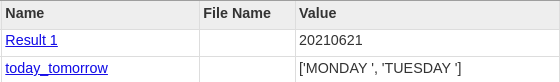
\includegraphics[width=.6\linewidth]{../output/78/1}
    \caption{(P14) Output}
\end{figure}




\subsection{Visualisations}

The \lstinline!Visualizer! is a module that is used for Visualizations, and supports a variety of ways to graph data. There are a variety of visualization formats available but the most common ones are shown here. Some are limited to 2 dimensional data models, whereas some are multidimensional and few are geospatial-based.

Here we plot the marks in a few subjects by the use of the visualizer module.

\lstinputlisting[caption={(P15) - Basic Visualizations}]{../source/79-vis.ecl}


Going to the standard output tab in ECL Watch gives us the data, but we can go to the `Resources tab to view the visualizations'.

(The default header is taken as `Dermatology' for some reason).

\begin{figure}[h]
    \centering
    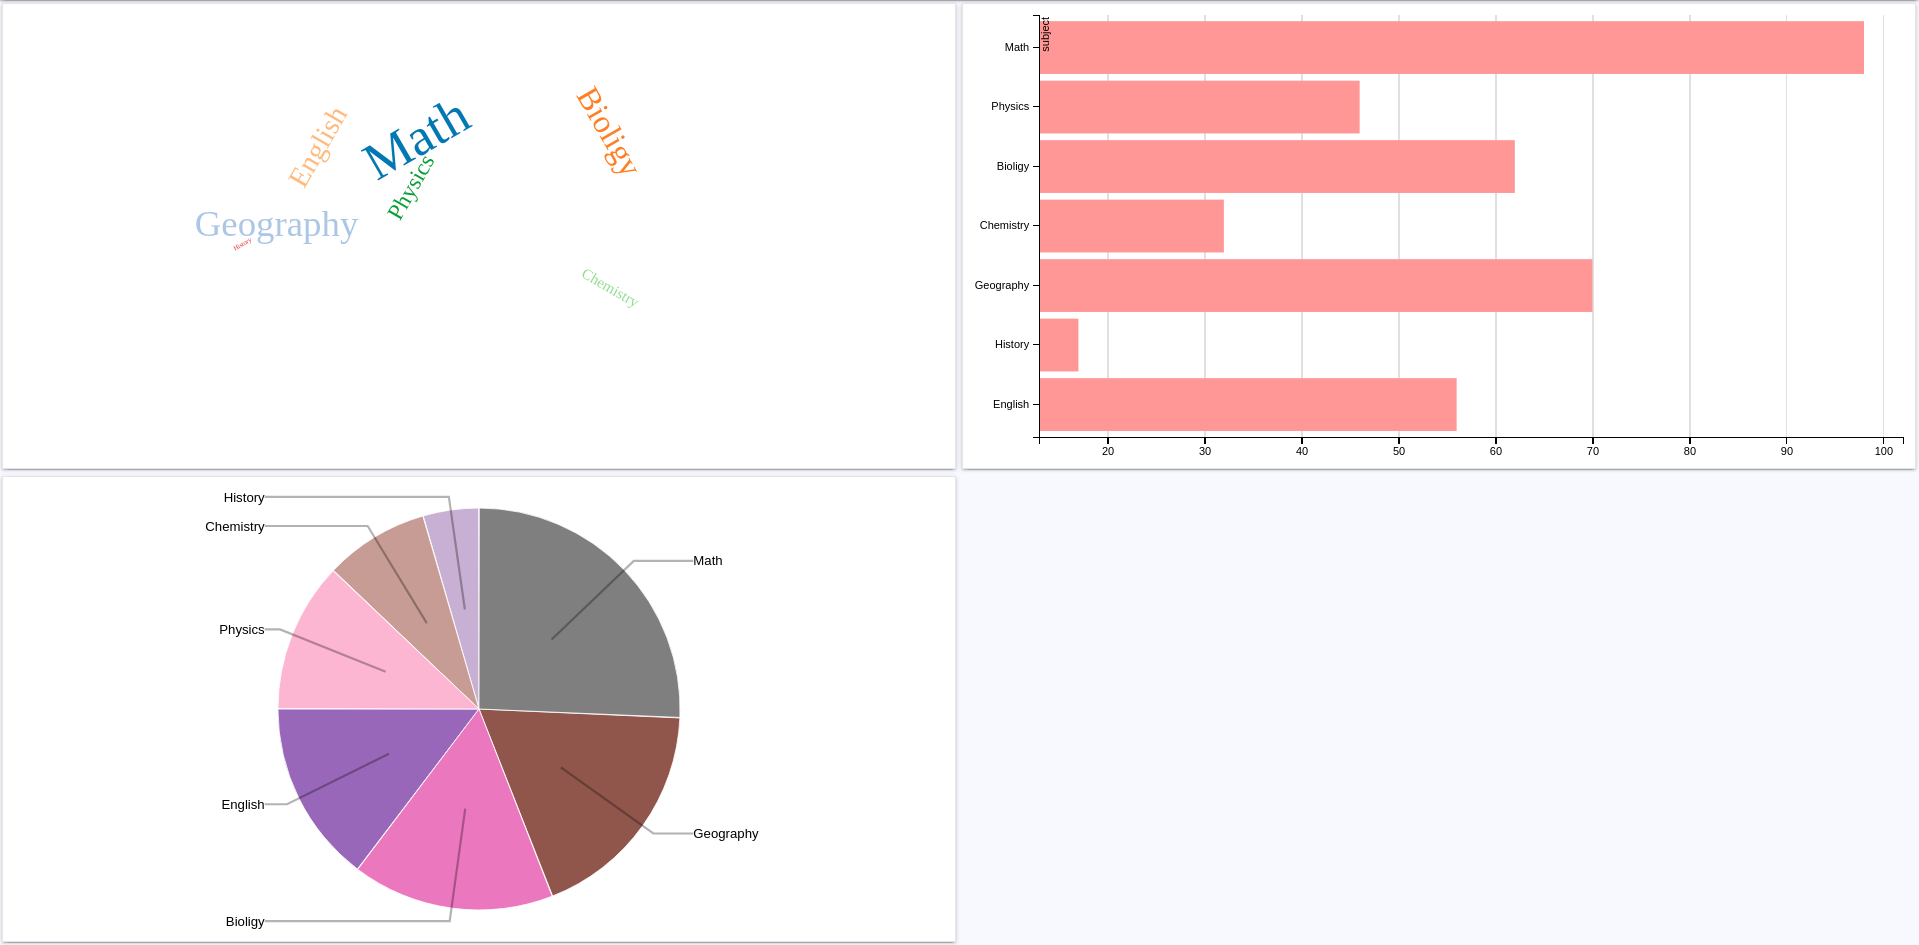
\includegraphics[width=.6\linewidth]{../output/79/1}
    \caption{(P15) Visualization}
\end{figure}




\chapter{Pre-Machine Learning}
\section{Techniques useful for Machine Learning}
\subsection[Dataset Shuffling]{(P16) Dataset Shuffling}

Dataset shuffling is a \textbf{very} important portion of data processing before feeding into machine learning models. This ensures even data distributions and is a good step to perform just before shuffling your dataset (up next).

Now how to shuffle? You can use \lstinline{RANDOM()} to obtain random values in an ECL Program. If this gives an idea, that's great! Adding a field with a value of \lstinline{RANDOM()} and sorting according to it, is a rather effective way to do shuffle a dataset in ECL.

\lstinputlisting[caption={(P16) Shuffle Dataset}]{../source/54-shuffle.ecl}

The output, looks as we would expect. The data has been shuffled. It is important to note that most people don't actually remove the id term, but start using it for an sequential serial id \#. This often goes hand in hand with the fact that HPCC Machine Learning modules expect a first column having a serial \# (Although this can be manually added in with a macro too).

\begin{figure}[h]
    \centering
    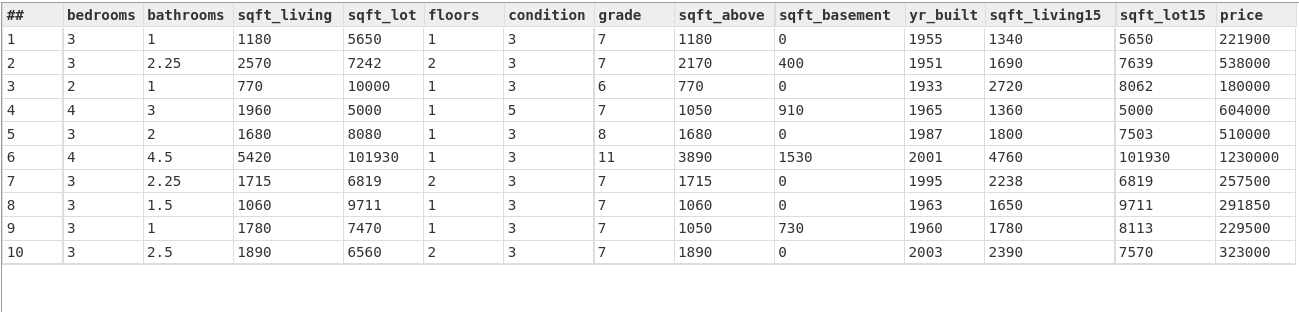
\includegraphics[width=\linewidth]{../output/54/default}
    \caption{Default output}
\end{figure}
\begin{figure}[h]
    \centering
    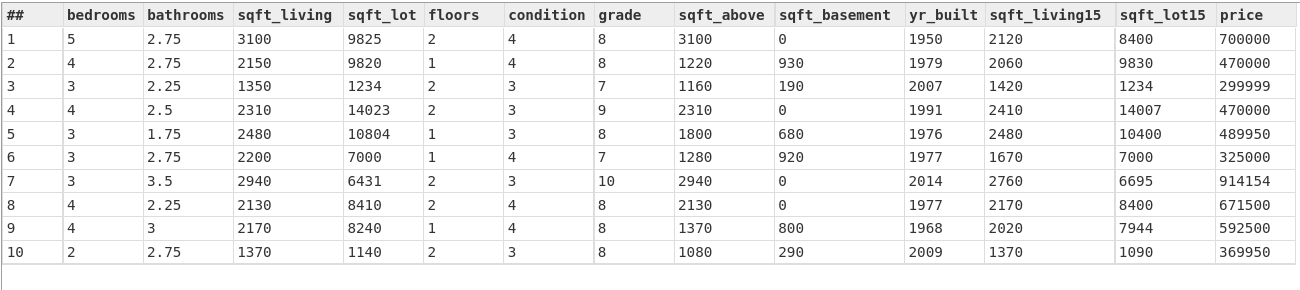
\includegraphics[width=\linewidth]{../output/54/shuffled}
    \caption{Shuffled output}
\end{figure}


\subsection[Dataset Splitting]{(P17) Dataset Splitting}

Dataset splitting is again an important step to working with Machine Learning. Usually, a dataset is split into 2/3 sections, and one set is the training set, and the other is the dev/testing set(s). Once a dataset has been randomized, it can be easily split.

\lstinputlisting[caption={(P17) Split Dataset}]{../source/55-split.ecl}

Here's what the outputs of the program looks:

\begin{figure}[h]
    \centering
    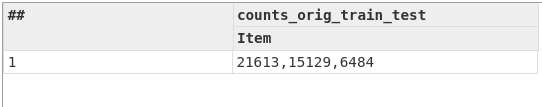
\includegraphics[width=.7\linewidth]{../output/55/counts}
    \caption{Counts $=>$ $6484+15129=21613$}
\end{figure}

\begin{figure}[h]
    \centering
    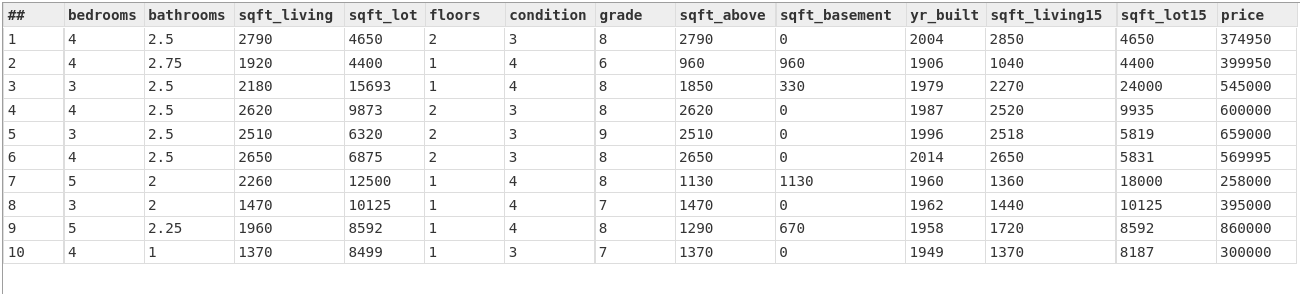
\includegraphics[width=\linewidth]{../output/55/original}
    \caption{Original}
\end{figure}

\begin{figure}[h]
    \centering
    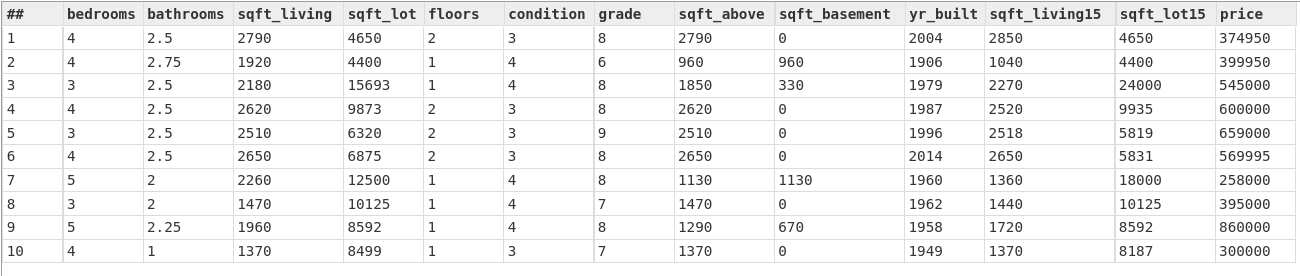
\includegraphics[width=\linewidth]{../output/55/train}
    \caption{Train set excerpt (It looks like the original)}
\end{figure}

\begin{figure}[h]
    \centering
    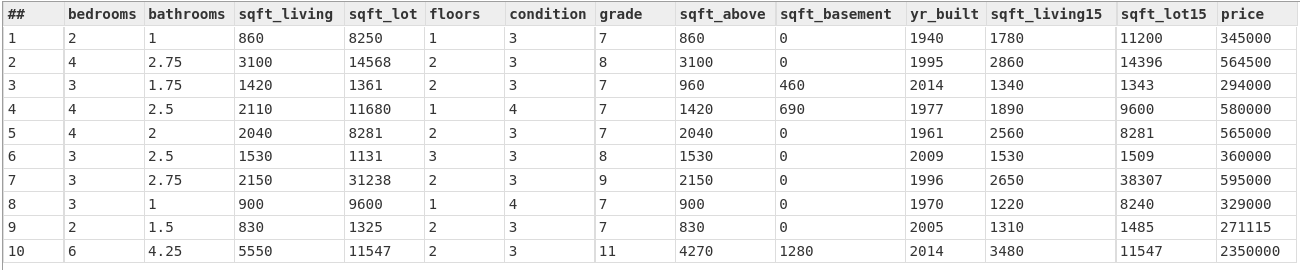
\includegraphics[width=\linewidth]{../output/55/test}
    \caption{Test set excerpt}
\end{figure}
